% !TEX TS-program = XeLaTeX
\documentclass{article}
\usepackage{fontspec}
\usepackage{amsmath,amssymb}
\usepackage{pifont}% http://ctan.org/pkg/pifont
\usepackage{tikz}
\usetikzlibrary{positioning, matrix, arrows.meta, shapes.geometric, calc,
  decorations.pathmorphing, decorations.pathreplacing, fit, shapes.multipart}
\usepackage{mathabx}
\usepackage{mathtools}
\usepackage{mathpartir}
\usepackage{fancyvrb}
\usepackage{stmaryrd}
\usepackage[normalem]{ulem} % for strikeout
\usepackage{listings}
\usepackage{semantic}          % for mathlig

\newcommand{\hide}[1]{}
\newcommand{\note}[2]{{\color{blue} #1}{\marginpar{\color{blue}AM}}}

\mathlig{->}{\mathbin{\shortrightarrow}}
\mathlig{-.}{\mathbin{\rightharpoonup}} % TODO remove these and use options instead

\defaultfontfeatures{Mapping=tex-text,Scale=MatchLowercase}

\begin{document}

\title{Lazy Sivaraman with Shaping}
\maketitle

\section{Setup and Notation}

\subsection{Abstract types}
We leave the following abstract:
\begin{itemize}
\item type \textit{pkt}, for packets 
\item type $n$, for node IDs 
\item type $s$, for node states
\item type \textit{rank}, for ordering payloads
\item type \textit{time}, for moments in time
\item type \textit{m}, for packet-specific metadata
\item type \textit{id}, for identifying metadata by index
\end{itemize}

\subsection{Derivative types leading to the configuration tree}

We can now build the following key items:
\begin{itemize}
\item type $p$ = Packet of ($\mathit{pkt} \times \mathit{id}$) | Pointer of ($n \times \mathit{id}$) 
\item type $q1$ = ($p \times \mathit{rank}$) PIFO, ordered by \textit{rank} 
\item type $q2 = (\mathit{time} \times \mathit{id})$ PIFO, ordered by \textit{time} 
\item type \textit{schedule}: $\mathit{time} -> p -> m -> s -> (\mathit{rank} \times s)$ 
\item type \textit{shape}: $\mathit{time} -> p -> m -> s -> (\mathit{time} \times s)$ 
\item type $\mathit{node\_info}:  (q1 \times q2 \times s \times \textit{schedule} \times \textit{shape})$
\item type $C: \{ \mathit{tree}: \mathit{node\_info} \text{ tree}; 
			\mathit{metastore}: m \text{ array} \}$ 
\end{itemize}

The ADT $p$ is read ``payload''. 
The PIFOs $q1$ and $q2$ are the scheduling and shaping queues respectively.
Next, \textit{schedule} is the type of scheduling functions; these compute a given 
payload's rank while possibly making edits to the given node's state.
Similarly, \textit{shape} is the type of shaping functions; these compute a payload's 
earliest requested release time while possibly making edits to the state. 
Both of these accept a \textit{time} input and may use it in their calculations.

\subsection{Navigating the tree}

The 5-tuple $\mathit{node\_info}$ is associated with each node in a tree. 
Unshaped nodes are given the trivial shaper, which just returns its first and third arguments. 
The tree, along with an array of metadata, comes together in a record
that is called a \textit{configuration} and has type \textit{C}.

It is helpful to be able to efficiently read and write the 5-tuple for a node,
and similarly with metadata:
\begin{itemize}
\item function \textit{read\_node}: $n -> C -> \mathit{node\_info}$ 
\item function \textit{write\_node}: $n -> \mathit{node\_info} -> C -> C$ 
\item function \textit{read\_meta}: $p -> C -> m$ 
\item function \textit{write\_meta}: $C -> \mathit{id} -> m -> C$ 
\end{itemize}

In addition, we require a few utilities that let us navigate the tree.
Interestingly, having these means that we do not strictly need the tree datastructure.
\begin{itemize}
\item function \textit{root\_index}: $C -> n$
\item function \textit{parent}: $n -> C -. n$
\item function \textit{nodes}: $C -> n~\mathit{list}$
\item function \textit{leaves}: $C -> n~\mathit{list}$
\item function \textit{haschildren}: $n -> C -> \mathbb{B}$
\item function \textit{children}: $n -> C -. n~\mathit{list}$
\end{itemize}


\subsection{A word on notation}

Going forward, we will continue to write the names of types in \textit{italics},
and we will also begin to write the name of the type in  \texttt{fixed-width} 
to refer to an \underline{instance} of that type. 
For example, when a method has \textit{time} as an argument
and uses \texttt{time} in its work, we assume that 
some (\texttt{time} : \textit{time}) was passed to it.


\section{Key Methods}

\subsection{Local push}

function \textit{local\_push}: 
$\mathit{time} -> p -> m -> (q1 \times q2 \times s \times \mathit{schedule} \times \mathit{shape}) -. \mathit{node\_info}$ 
\begin{enumerate}
\item $(\mathtt{r}, \mathtt{s'}) \coloneqq \texttt{schedule time p m s}$
\item $\mathtt{q1'} \coloneqq \mathit{enqueue}~\mathtt{q1}~(\mathtt{p}, \mathtt{r})$
\item $(\mathtt{t}, \mathtt{s''}) \coloneqq \texttt{shape time p m}~\mathtt{s'}$ 
\item $\mathtt{q2'} \coloneqq \mathit{enqueue}~\mathtt{q2}~(\mathtt{t}, \mathit{get\_id}~\mathtt{p}) $
\item return $(\mathtt{q1'}, \mathtt{q2'}, \mathtt{s''}, \mathtt{schedule}, \mathtt{shape})$
\end{enumerate}

\hide{The boolean argument is \texttt{isroot}, which says whether the node 
we are working on is the root node of the tree. We use this exactly 
as seen in step 3 above, because we want to keep the root's shaping queue empty.
We will discuss this further in \S3.2.}
\noindent Note the use of the \textit{enqueue} method from the underlying PIFO library.
This is partial because the relevant queues may be at capacity, causing \textit{enqueue} to fail.
We leave the method ``$\mathit{get\_id: p -> \mathit{id}}$'' abstract.


\subsection{Local push wrapped}

function \textit{local\_push\_wrapped}: $\mathit{time} -> p -> n -> C -. C$ 

This is a simple convenience. 
Read the 5-tuple associated with \texttt{n} from \texttt{C}'s tree and 
extract \texttt{p}'s metadata from the metastore.
Invoke \textit{local\_push} with this information 
and write the local change back into \texttt{C}'s tree. 
Pass $\mathtt{time}$ unchanged.

\subsection{Local pop wrapped}

function \textit{local\_pop1\_wrapped}: $n -> C -. ((p \times \mathit{rank}) \times C)$  \\
function \textit{local\_pop2\_wrapped}: $n -> C -. (\mathit{time} \times C)$ 

Similarly, it is convenient to have ``wrapped'' versions of \textit{pop}. 
Read node details from the configuration tree, perform a basic PIFO \textit{pop} operation on q1 or q2 respectively,
and then write local changes back into the tree.
Again, these are partial because the underlying PIFO \textit{pop} operation can fail.

\subsection{Housekeep minimal}

function \textit{housekeep\_minimal}: $\mathit{time} -> n -> C -> C~\mathtt{option}$ 

\begin{enumerate}
\item $(\_, \mathtt{q2}, \_, \_, \_) \coloneqq \mathit{read\_node}~\mathtt{n~C}$
\item If ($\mathtt{q2} = \textit{nil}$ or $\mathit{fst~(peek~\mathtt{q2})} > \mathtt{time}$, return \texttt{None}
\item $((\_, \mathtt{id}), \mathtt{C'}) \coloneqq \textit{local\_pop2\_wrapped}~\mathtt{n~C}$
\item $\text{If } \mathtt{n} = \mathit{root\_index}~\mathtt{C},~\text{return}~(\mathtt{Some~C'}).$
\item return $\mathit{local\_push\_wrapped~time}~(\text{Pointer } \mathtt{(n, id)})~(\textit{parent } \mathtt{n~C'}) ~\mathtt{C'}$
\end{enumerate}

The return type is an \texttt{option}; this allows us to signal to the caller
of this method if any progress was made.
The method \textit{peek} is from the underlying PIFO library. 
If we get to step 3, we know we can try to make progress.
We pop off the head of \texttt{q2}, which is known to be ready.
If we are ourselves the root of the tree, we are done and can return.
If not, we push into our parent (\textit{parent}~$\mathtt{n~C'}$) 
a pointer to ourselves (Pointer~\texttt{n}).
Note that \textit{local\_push\_wrapped} can fail because of the parent being at capacity.  
Even so, \underline{we} don't fail; we just scrap our work and return \texttt{None}.

\note{Nate mentioned an opportunity for cleanup thanks to the Option return type, 
but I've forgotten what it was. Sorry, could I get a reminder?}

\subsection{Can housekeep}

$\mathit{can\_housekeep_{time}}$ is a relation over $\mathit{C} \times \mathit{C}$
with respect to some \texttt{time}. 
The pair of configurations ($\mathtt{C_1}, \mathtt{C_2}$) 
is in the relation if
$$\exists \mathtt{n}.~\mathtt{n} \in (\mathit{nodes}~\mathtt{C}) \wedge \mathit{housekeep\_minimal}~\mathtt{time~n~C_1} = \mathtt{Some~C_2}$$

\note{Hm, I'm not sure if I got this totally right either.
The business of fixing some time seems a bit odd, and I'm not sure how to 
state this in the negative, i.e. ``there is no more housekeeping to be done''.}

\subsection{Fully housekept}

function \textit{fully\_housekept}: $\mathit{time} -> C -> \mathbb{B}$

\note{A different take, probably not what we want:}

$$\forall \mathtt{n}.~\mathtt{n} \in (\mathit{nodes}~\mathtt{C}) -> \mathit{housekeep\_minimal}~\mathtt{time~n~C} = \mathtt{None}$$


\subsection{Pop}

function \textit{pop\_helper}: $n -> C -. (\mathit{pkt}, C)$
\begin{enumerate}
\item $\mathtt{((v,\_), C')} \coloneq \mathit{local\_pop1\_wrapped}~\mathtt{n~C}$
\item \texttt{match v with} Packet ($\mathtt{pkt}, \_) -> (\mathtt{pkt}, \mathtt{C'})$ | Pointer ($\mathtt{n}, \_) -> \mathit{pop\_helper}~\mathtt{n~C'}$
\end{enumerate}

\noindent function \textit{pop}: $C -. (\mathit{pkt}, C)$

\textit{pop\_helper} (\textit{root\_index} \texttt{C}) \texttt{C}.

\vspace{1em}
\noindent Both of these are partial: the former because \textit{local\_pop1\_wrapped} is,
the latter because it calls the former. 
If passed a tree that is known to be fully housekept with respect to some \textit{time}, 
\textit{pop} gives the highest-priority packet that was ``ripe'' at that time. 

\subsection{Push}

function \textit{push}: $\mathit{time} -> \mathit{pkt} -> n -> C -. C$ 
\begin{enumerate}
\item $\mathtt{id} = \mathit{new\_id~()}$
\item $\mathtt{C'}$ = \textit{local\_push\_wrapped} $\mathtt{time}$ (\text{Packet} ($\mathtt{pkt, id}$)) $\mathtt{n~C}$
\item $\mathtt{C''} = \mathit{write\_meta}~\mathtt{C' ~ id}~(\mathit{packet\_to\_meta}~\mathtt{pkt})$
\item return $\mathtt{C''}$
\end{enumerate}


\section{Notes and Open Questions}

\subsection{Cardinality}

In both shaped and unshaped nodes, $\mathtt{q2}$ tells us
how many payloads from this node have not yet been propagated upwards to 
the parent node.

We can define the cardinality of a node as:
$$|n| \coloneqq |\mathtt{q1}_n| - |\mathtt{q2}_n|$$

We can place the following correctness condition:  
$$\forall n, C.~\mathit{haschildren~n~C} -> |n| \le \sum_{n' \in (\mathit{children~n~C})}^{} |n'| $$

\subsection{Size, packet dropping}

Each node in the tree can be initialized with arrays \texttt{q1} and \texttt{q2} of any size. 
We don't worry about the size of the tree overall. 
Rather, individual \textit{enqueue} operations into \texttt{q1} or \texttt{q2} may fail, 
in which case the top-level operation (\textit{push} or \textit{housekeep\_minimal}) 
that triggered the offending \textit{enqueue} will fail
without altering the tree. When a \textit{push} fails in this way, the incoming packet is dropped.


\subsection{Shaper and scheduler in lockstep?}
 
In unshaped nodes, we still do use $\mathtt{q2}$. 
For these nodes it doesn't matter if the two queues are in lockstep, since 
$\mathtt{q2}$ is used essentially as counter.

In shaped nodes, one may want to keep the queues in lockstep. 
Here's an example of bad behavior when the scheduling function and 
the shaping function give packets different orderings.

Suppose there exist packets $a$ and $b$ and nodes $P$ and $C$.
$P$ is the parent of $C$.
The node $C$ has the scheduling function $\mathit{sched_{C}}$
such that
$\mathit{sched_{C}~a} = 1$ and $\mathit{sched_{C}~b} = 2$. 
Lower is ``better'', i.e. $a$ has higher priority than $b$.
Further, $C$ has the shaping function $\mathit{shape_{C}}$
such that $\mathit{shape_{C}~a}=9$ and $\mathit{shape_{C}~b}=7$.
So~$a$ should be emitted no earlier than time $9$ and $b$ no earlier than time $7$.

In the discussion below, I've tried to follow the terminology shown in Fig 5 of the
SIGCOMM paper.

\begin{center}
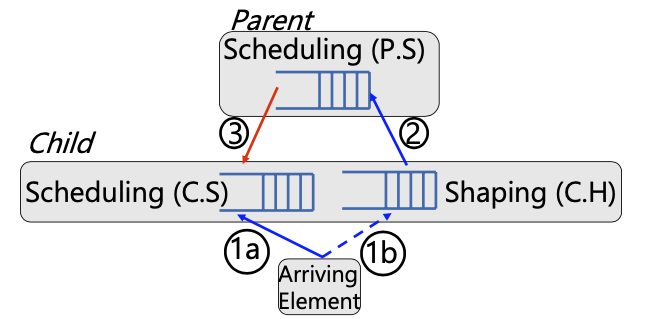
\includegraphics[width=0.4\textwidth]{siv_fig5}
\end{center}

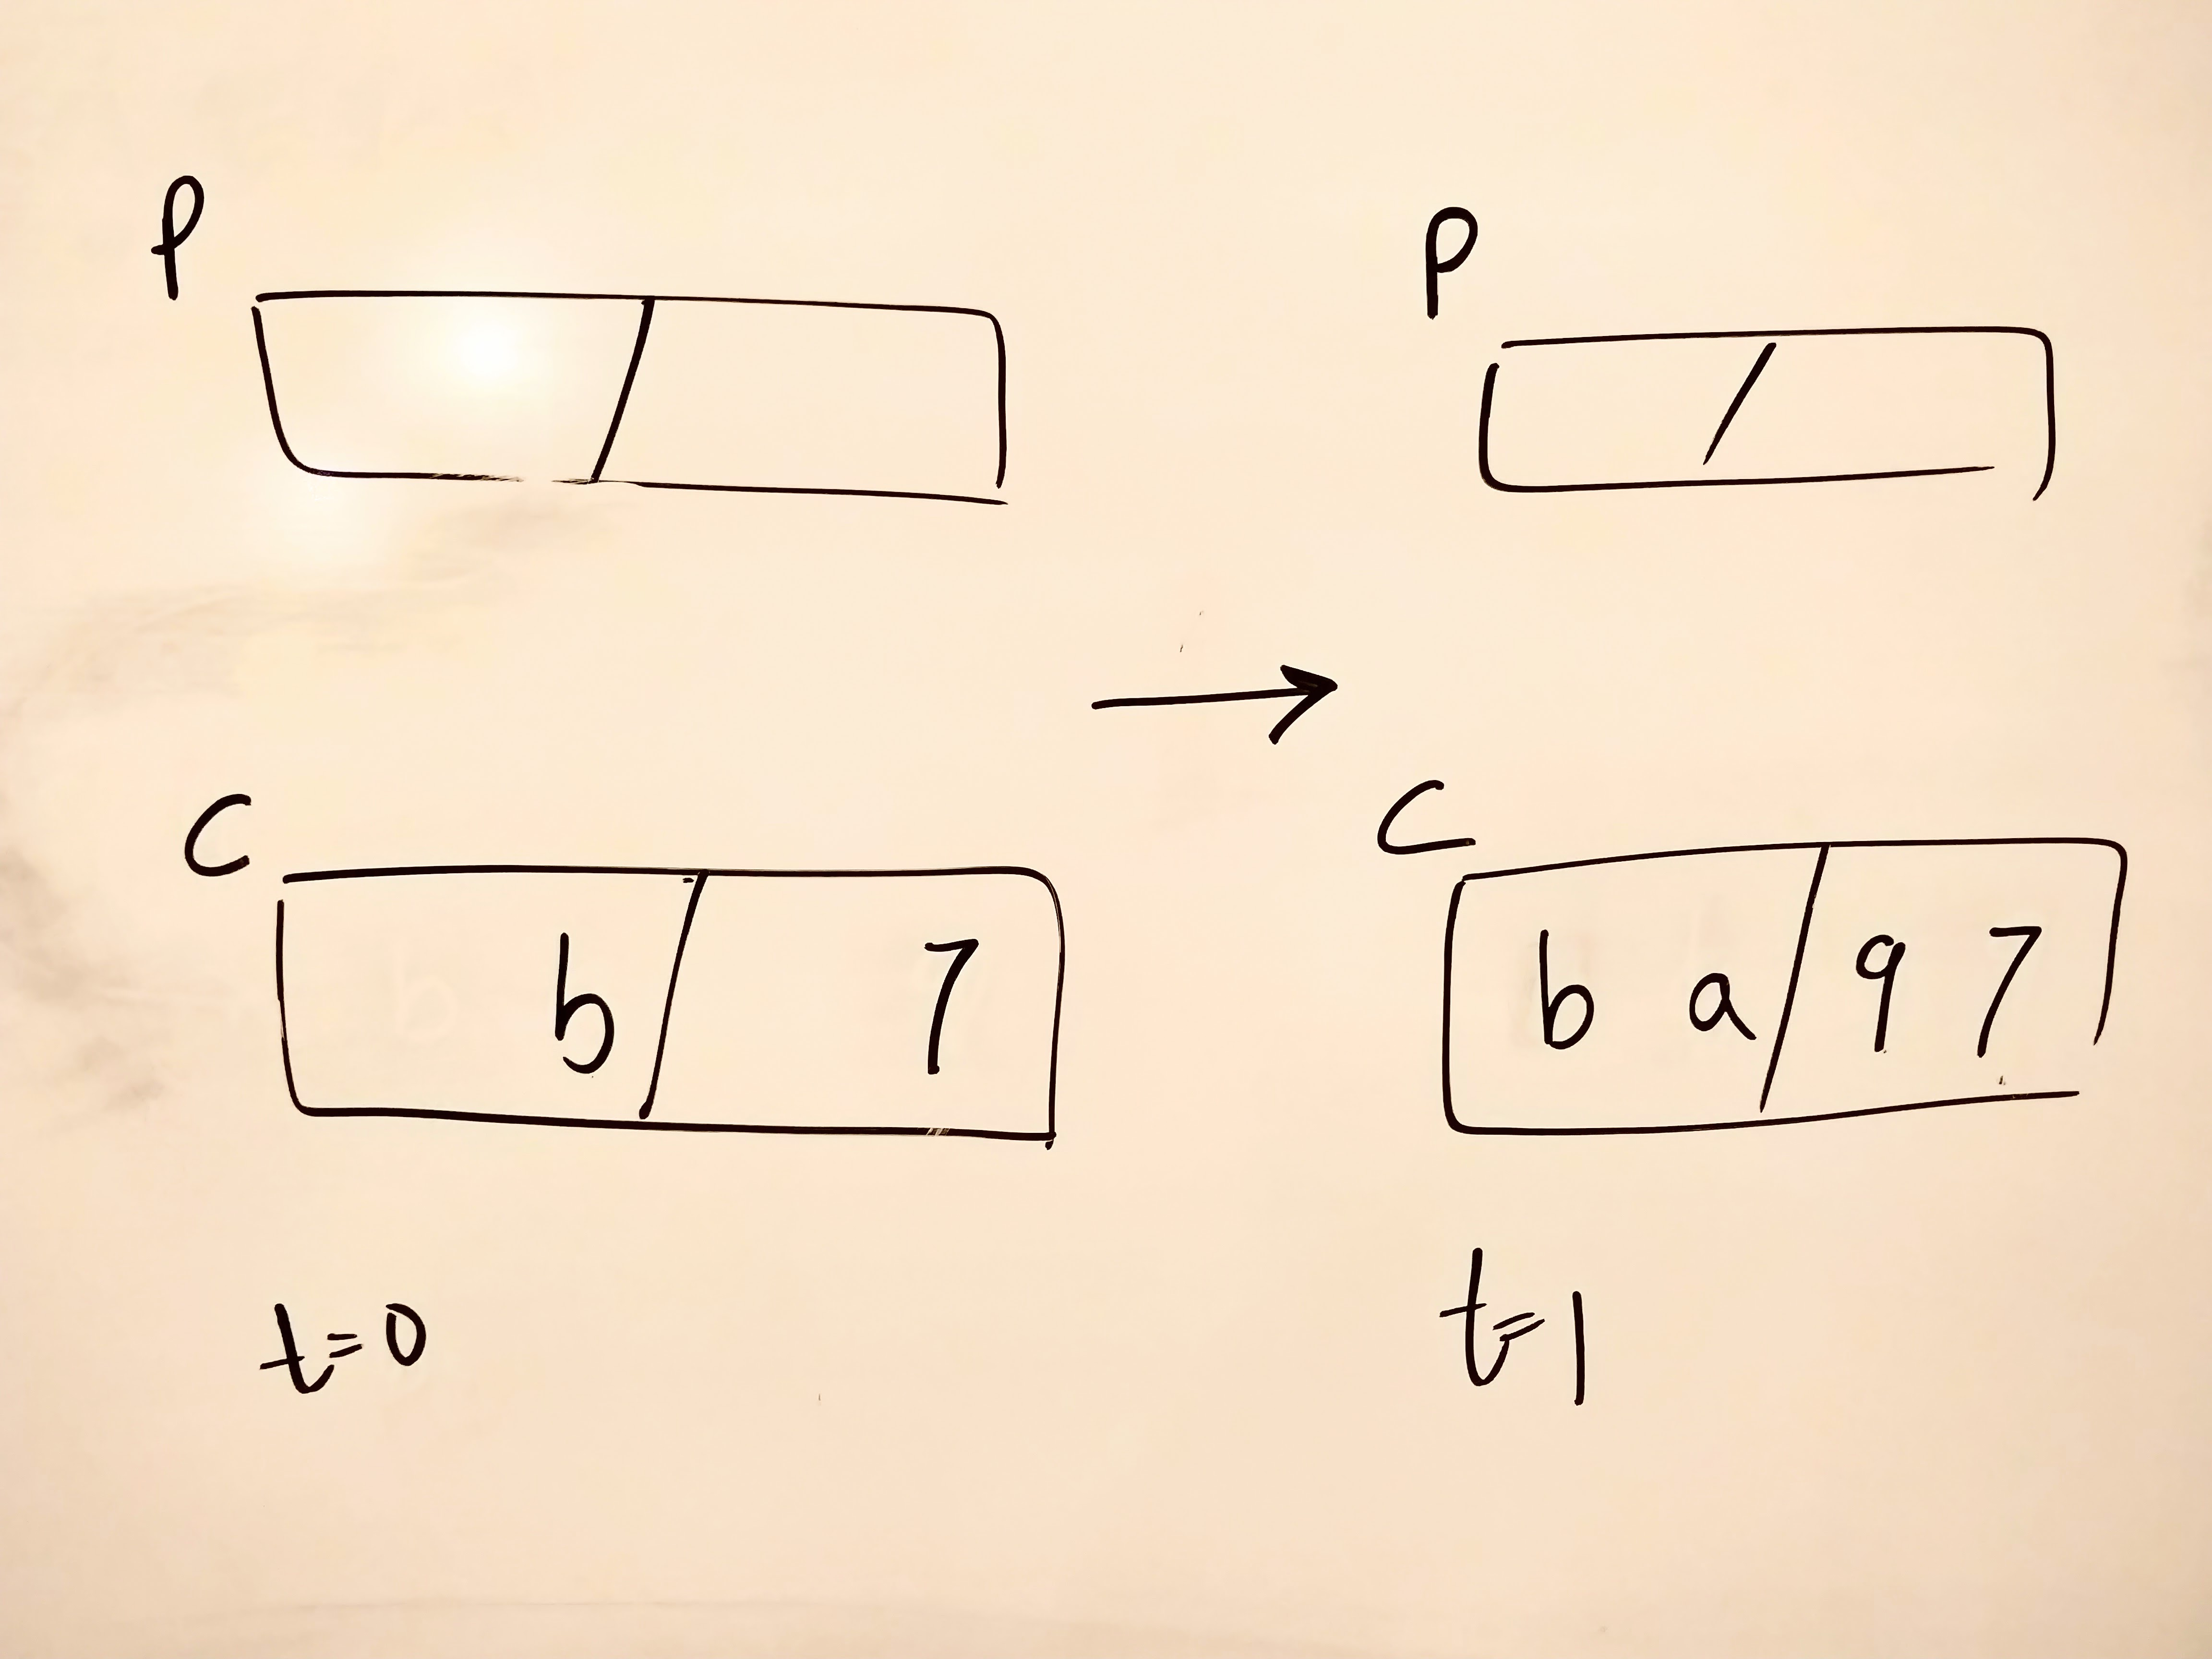
\includegraphics[width=0.4\textwidth]{shaped_badly_1}
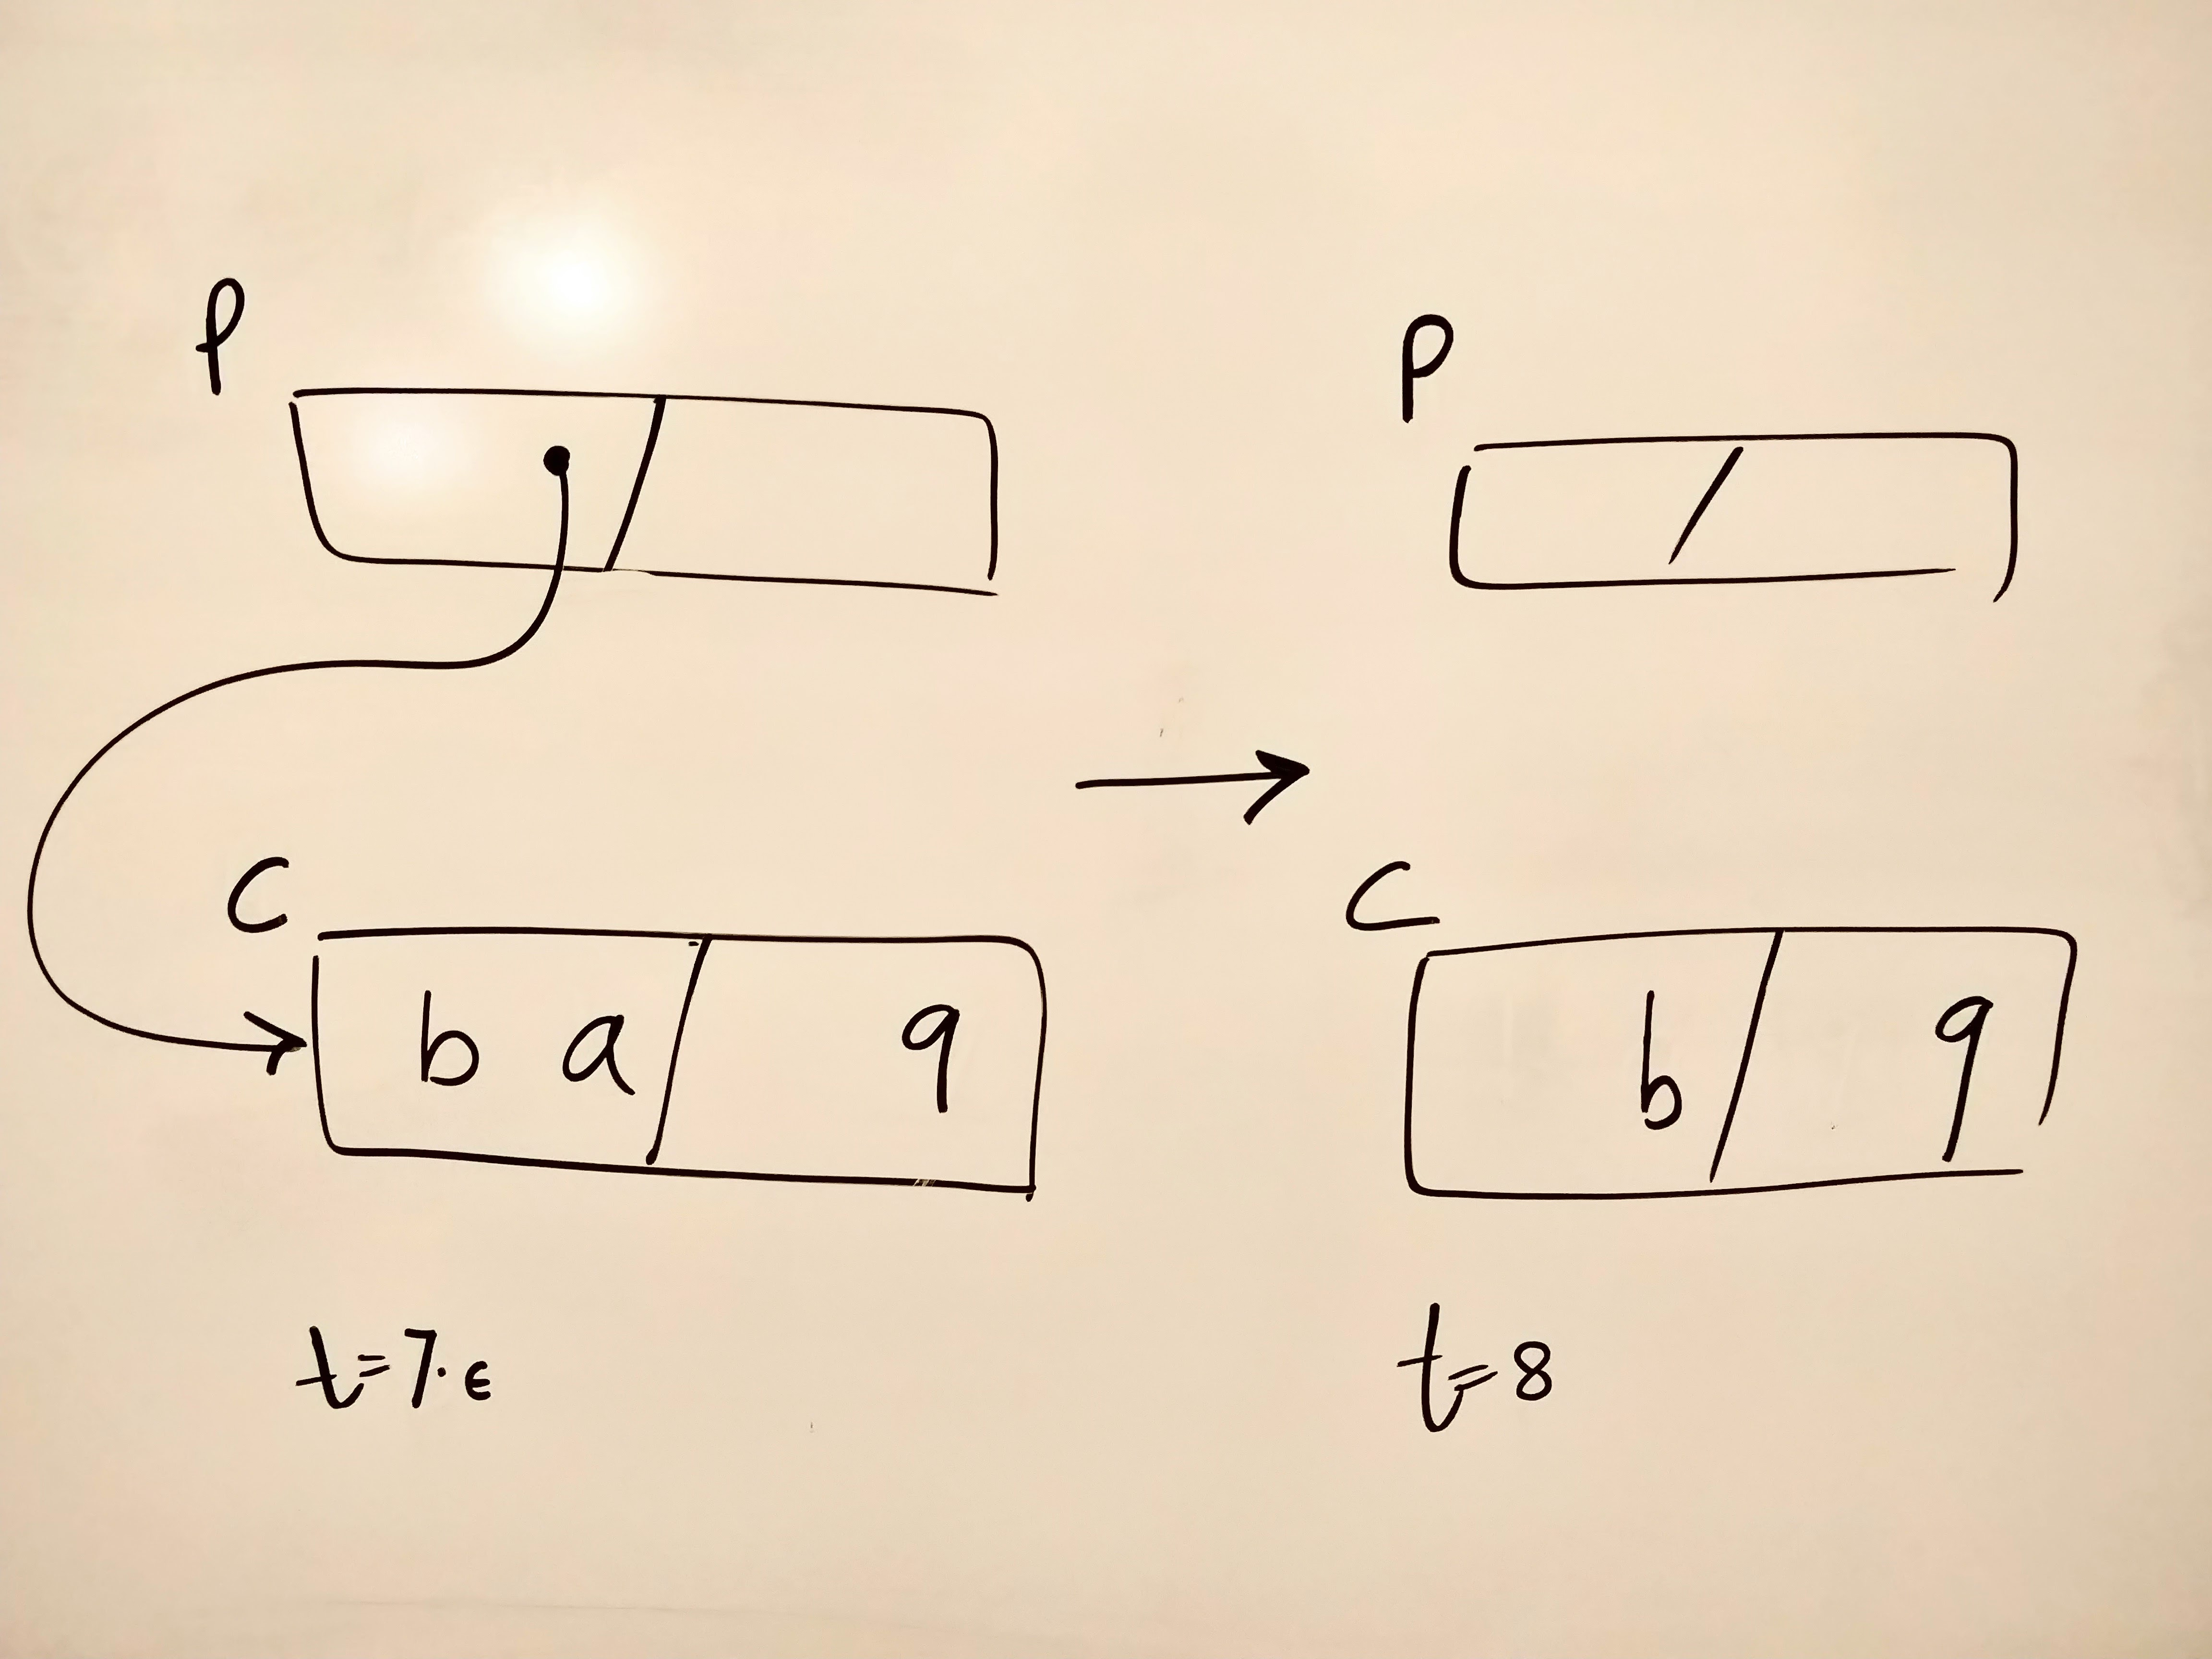
\includegraphics[width=0.4\textwidth]{shaped_badly_2}

The following operations occur:
\begin{itemize}
\item Time 0: $b$ is enqueued into $C$. 
This causes $b$ to be added to C.S with rank~$2$, and a reference to C.S 
to be enqueued into C.H with release time~$7$.
\item Time 1: $a$ is enqueued into $C$. 
This causes $a$ to be added to C.S with rank~$1$, and a reference to C.S 
to be enqueued into C.H with release time~$9$.
\item Time 7: \textit{housekeep\_minimal} is called on C. 
An element of C.H is indeed ready! Dequeue it, and enqueue it into 
$P$'s scheduling queue P.S.
\item Time 8: Pop is called. $P$ sees that it has a ready reference, so it calls 
pop on C.S. The top-priority item in C.S is $a$, so it is popped.
\end{itemize}

This behavior is doubly problematic: $a$ was released before its requested 
release time, and $b$ will be forced to wait until time $9$. 
Of course one can cook up a nastier situation where $\mathit{shape_{C}~a}$ 
was not $9$ but $9000$, in which case 
$a$ will now be \emph{very} early and $b$ \emph{very} late.
 
In essence $a$ was released at the requested release time of $b$
because it had a better rank than $b$.
You and I know that the reporting to $P$ at time~$7$ was done because $b$ 
was ready, not $a$. 
But $P$ is not working at the per-packet level; it is essentially just working with cardinalities. 
It learns that one more packet is ready in $C$, so it adds one more reference to $C$.

\subsection{Payload length}
Scheduling and shaping transactions often need to access a payload's length; 
see Figs 2c and 4c from the SIGCOMM paper. 
For a Packet payload the answer is obvious, but for an Pointer payload it is more subtle. 
Sivaraman handles this via a metadata field, essentially remembering the length of the 
packet that the Pointer points to. 
However, this seems risky/wrong: as we have discussed, an Pointer points not to 
a packet but to a node. Its target packet can change.

\end{document}
